\documentclass[10pt,aspectratio=169]{beamer}

% All the boilerplate is in ccaslides.sty
% Note that this also pulls in a custom vogtwidebar.sty
\usepackage{ccaslides}

\author{Ji\v{r}\'i Lebl}

\institute[OSU]{%
Departemento pri Matematiko de Oklahoma {\^S}tata Universitato}

\title{Cultivating Complex Analysis: Introduction}

\date{}

\begin{document}

\begin{frame}
\vspace*{-0.5in}
\titlepage

\vspace*{-0.5in}
\hspace*{-0.2in}
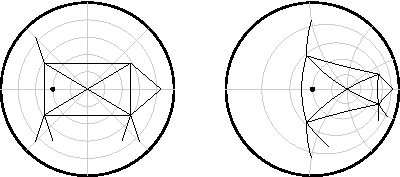
\includegraphics[width=1.9in]{../figures/varphiplot.pdf}

\vspace*{-1.0in}
\hspace*{1.84in}%
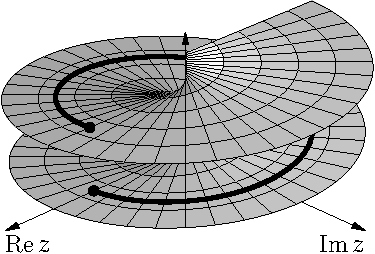
\includegraphics[width=1.9in]{../figures/arggraph2.pdf}%

\vspace*{-1.1in}
\hspace*{3.8in}%
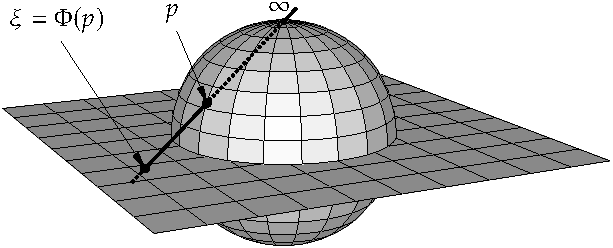
\includegraphics[width=1.9in]{../figures/riemannsphere.pdf}%
\end{frame}

\begin{frame}
Goal is to present a standard graduate one semester
course on Complex Analysis.

\medskip
\pause

The course follows closely the freely downloadable book:

\medskip

Ji\v{r}\'i Lebl,
\emph{Cultivating Complex Analysis: Working the Complex Field,}
\url{https://www.jirka.org/ca/}

\medskip

An inexpensive paperback copy is available.

\medskip
\pause

These slides and the book is available in \LaTeX\ form for easy modification
under a creative commons license.

\medskip
\pause

My goal is to record a lecture every week or two for the forseeable future.


\end{frame}

\begin{frame}
Prerequisites:

\medskip
\pause

Basic undergraduate analysis

\medskip
\pause

\quad Metric spaces

\pause

\quad Riemann integral, interchange of uniform limits, derivative
under the integral, Fubini

\pause

\quad Derivative in several variables, namely for functions from $\R^2$ to
$\R^2$

\pause
\medskip

Linear algebra, and some basic abstract algebra

\pause
\medskip

Overall experience with proofs

\pause
\medskip

No courses that are usually considered graduate courses are required.
Explicitly, Lebesgue integral and measure theory is not needed.

\end{frame}

\begin{frame}
Outline of the course (chapters in the book):

\begin{itemize}
\item
The Complex Plane (chapter 1)
\begin{itemize}
\item Basic geometry of the complex plane,
Riemann sphere,
linear fractional transformations.
\end{itemize}

\pause
\item Holomorphic and Analytic Functions (chapter 2)
\begin{itemize}
\item
Holomorphic functions (complex differentiability, Cauchy--Riemann equations),
power series and analytic functions, the exponential, identity theorem.
\end{itemize}

\pause
\item Line Integrals and Rudimentary Cauchy Theorems (chapter 3)
\begin{itemize}
\item
Line integrals, basic versions of Cauchy theorems, Cauchy--Goursat,
Cauchy formula for a disc,
holomormphic functions are analytic,
maximum principle,
Cauchy estimates,
Liouville's theorem,
fundamental theorem of algebra,
convergence of holomorphic functions,
Schwarz's lemma and automorphisms of the disc.
\end{itemize}

\pause
\item The Logarithm and Cauchy (chapter 4)
\begin{itemize}
\item
Defining the logarithm via continuation,
winding numbers, homology version of Cauchy,
simply connected domains,
Laurent series.
\end{itemize}

\pause
\item Counting Zeros and Singularities (chapter 5)
\begin{itemize}
\item
Zeros, isolated singularities, the residue theorem,
the argument principle,
Rouch\'e, Hurwitz,
open mapping theorem, inverses are holomorphic.
\end{itemize}

\pause
\item Montel and Riemann (chapter 6)
\begin{itemize}
\item
Arzel\`a--Ascoli, Montel, Riemann mapping theorem.
\end{itemize}

\end{itemize}
\end{frame}

\begin{frame}
\begin{itemize}

\item Harmonic Functions (chapter 7)
\begin{itemize}
\item
Basic properties, Dirichlet problem in a disc and the Poisson kernel,
mean-value property, Harnack's inequality and principle,
extending harmonic functions past singularities/boundaries.
\end{itemize}

\pause
\item Weierstrass Factorization (chapter 8)
\begin{itemize}
\item
Infinite products, factorization of holomorphic functions.
\end{itemize}

\pause
\item Rational Approximation (chapter 9)
\begin{itemize}
\item
Polynomial approximation, Runge's theorem, polynomial hull, Mittag-Leffler.
\end{itemize}

\pause
\item Analytic continuation (chapter 10)
\begin{itemize}
\item
Schwarz reflection principle, analytic continuation along paths, Monodromy
theorem.
\end{itemize}
\end{itemize}

\end{frame}

\begin{frame}
Connections to prior knowledge rather than reinventing the wheel

\medskip
\pause

Complex differentiable versus (real) differentiable

\medskip
\pause

$(z,\bar{z})$ versus $(x,y)$
\end{frame}

\end{document}
